\documentclass[landscape]{standalone}
\usepackage{tikz}
\usetikzlibrary{calc,intersections,through,backgrounds,decorations.pathreplacing,decorations.markings,positioning}
\usepackage{graphicx}
\usepackage{amsmath}
\newcommand*\dif{\mathop{}\!\mathrm{d}}

\def\centerarc[#1](#2)(#3:#4:#5)% [draw options] (center) (initial angle:final angle:radius) 
{ \draw[#1] ($(#2)+({#5*cos(#3)},{#5*sin(#3)})$) arc (#3:#4:#5);}

\begin{document}
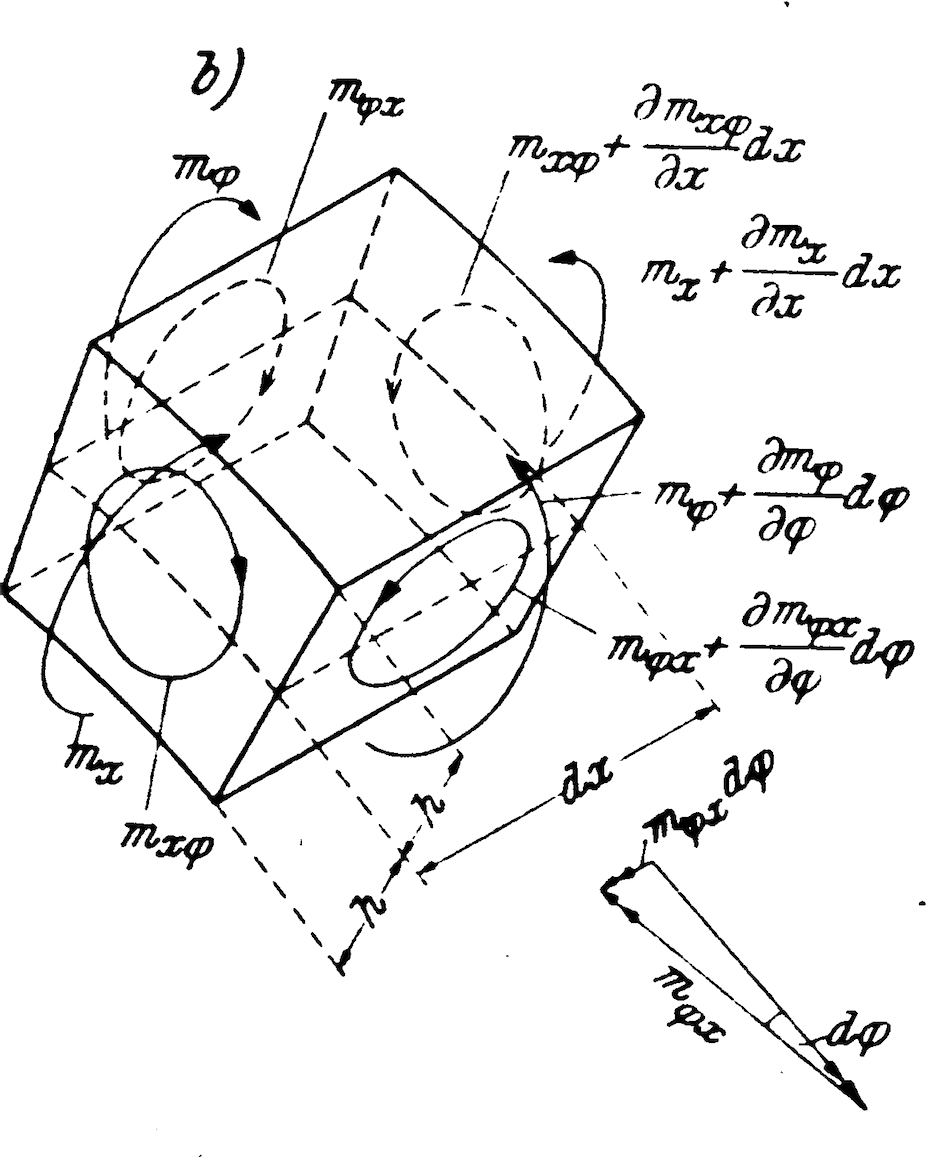
\includegraphics[width=6cm]{sr}\hfill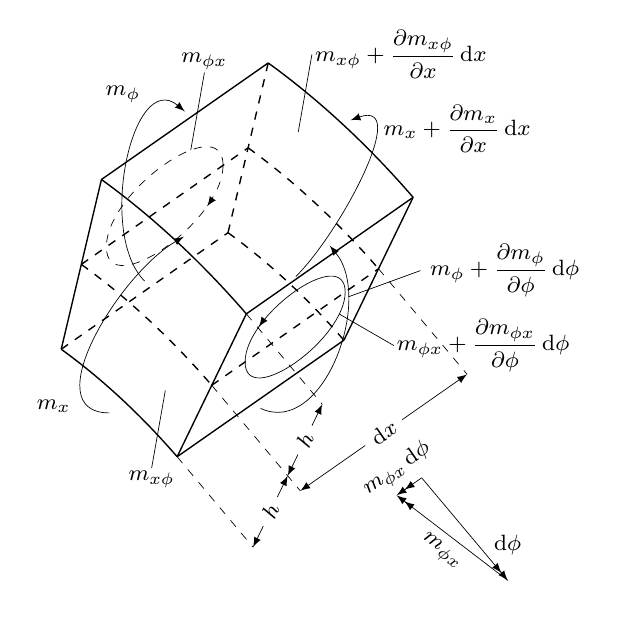
\begin{tikzpicture}[>=latex,line width=0.5pt,thinny/.style={line width=0.25pt},font={\footnotesize}]
% anterior face
\begin{scope}[xslant=0.35,yslant=-0.7]
\draw[] ($(0,0)+({10*cos(97)},{10*sin(97)})$) node (tl1) {} arc (97:83:10) node (tr1) {};
\draw[dashed] ($(0,0)+({9*cos(97)},{9*sin(97)})$)   node (cl1) {} arc (97:83:9)  node (cr1) {};
\draw[] ($(0,0)+({8*cos(97)},{8*sin(97)})$)   node (bl1) {} arc (97:83:8)  node (br1) {};
\draw[] (bl1.center) -- (tl1.center);
\draw[] (br1.center) -- (tr1.center);
\centerarc[->,thinny](0,9)(410:45:0.75)
\node[] (mxl) at ($(0,9)+({0.75*cos(-45)},{0.75*sin(-45)})$) {};
\end{scope}
% posterior face
\begin{scope}[xslant=0.35,yslant=-0.7,shift={(1.6,2.6)}]
\draw[] ($(0,0)+({10*cos(97)},{10*sin(97)})$) node (tl2) {} arc (97:83:10) node (tr2) {};
\draw[dashed] ($(0,0)+({9*cos(97)},{9*sin(97)})$)   node (cl2) {} arc (97:83:9)  node (cr2) {};
\draw[dashed] ($(0,0)+({8*cos(97)},{8*sin(97)})$)   node (bl2) {} arc (97:83:8)  node (br2) {};
\draw[dashed] (bl2.center) -- (tl2.center);
\draw[] (br2.center) -- (tr2.center);
\centerarc[->,dashed,thinny](0,9)(220:585:0.75)
\node[] (mxr) at ($(0,9)+({0.75*cos(135)},{0.75*sin(135)})$) {};
\end{scope}

% lateral faces
\begin{scope}[]
\draw[] (tr1.center) -- (tr2.center);
\draw[] (tl1.center) -- (tl2.center);
\draw[] (br1.center) -- (br2.center);
\draw[dashed] (bl1.center) -- (bl2.center);
\draw[dashed] (cr1.center) node (ar) {} -- node (cr) {} (cr2.center) node (br) {};
\draw[dashed] (cl1.center) node (al) {} -- node (cl) {} (cl2.center) node (bl) {};
\end{scope}
\path[thinny] ($(br)!0.4!(cr)$) edge[out=90,in=90,{postaction={decorate,decoration={markings,mark=at position .75 with {\arrow{latex}}}}}] ($(ar)!0.4!(cr)$); 
\path[thinny] ($(ar)!0.4!(cr)$) edge[out=-90,in=-90,{postaction={decorate,decoration={markings,mark=at position .85 with {\node (mzr) {};}}}}] ($(br)!0.4!(cr)$); 
\path[dashed,thinny] ($(bl)!0.3!(cl)$) edge[out=90,in=90,{postaction={decorate,decoration={markings,mark=at position .25 with {\node (mzl) {};}}}}] ($(al)!0.3!(cl)$); 
\path[dashed,thinny] ($(bl)!0.3!(cl)$) edge[out=-90,in=-90,{postaction={decorate,decoration={markings,mark=at position .25 with {\arrow{latex}}}}}] ($(al)!0.3!(cl)$); 

\begin{scope}[dashed,thinny]
\draw[] (tr1.center) -- ++(-50:1.5) node (ht) {};
\draw[] (br1.center) -- ++(-50:1.5) node (hb) {};
\draw[] (cr1.center) -- ++(-50:1.75) node (hc1) {};
\draw[] (cr2.center) -- ++(-50:1.75) node (hc2) {};
\end{scope}

\begin{scope}[<->,thinny,every node/.style={fill=white,sloped}]
\draw (hb.center) -- node {$h$} ($(hb)!0.5!(ht)$);
\draw ($(hb)!0.5!(ht)$) -- node {$h$} (ht.center);
\draw (hc1.center) -- node {$\dif x$} (hc2.center);
\end{scope}

\begin{scope}[thinny,inner sep=1pt]
\draw (mxl.center) -- ++(-100:1) node[anchor=north] {$m_{x\phi}$};
\draw (mxr.center) -- ++(80:1) node[anchor=west] {$m_{x\phi}+\dfrac{\partial m_{x\phi}}{\partial x}\dif x$};
\draw (mzl.center) -- ++(80:1) node[anchor=south] {$m_{\phi x}$};
\draw (mzr.center) -- ++(-30:0.8) node[anchor=west] {$m_{\phi x}+\dfrac{\partial m_{\phi x}}{\partial \phi}\dif\phi$};
\end{scope}

\node (hbr) at ($(br1)!0.5!(br2)$) {};
\node (htr) at ($(tr1)!0.5!(tr2)$) {};
\node (hbl) at ($(bl1)!0.5!(bl2)$) {};
\node (htl) at ($(tl1)!0.5!(tl2)$) {};
\node (hbb) at ($(br1)!0.5!(bl1)$) {};
\node (htb) at ($(tr1)!0.5!(tl1)$) {};
\node (hbt) at ($(br2)!0.5!(bl2)$) {};
\node (htt) at ($(tr2)!0.5!(tl2)$) {};

\path[thinny,->] (hbr.south) edge[out=-25,in=-50] node[inner sep=0,text width=0pt,near end] (mphipa) {} (htr.north);
\path[thinny,->] (hbl.north) edge[out=135,in=140] node[near end,anchor=south east] {$m_\phi$} (htl.north);
\draw[thinny] (mphipa) -- ++(20:1) node[anchor=west] {$m_{\phi}+\dfrac{\partial m_{\phi}}{\partial \phi}\dif\phi$};
\path[thinny,->] (hbt.north east) edge[out=45,in=20] node[near end,anchor=west] {$m_x+\dfrac{\partial m_x}{\partial x}\dif x$} (htt.north east);
\path[thinny,->] (hbb.south west) edge[out=180,in=210] node[anchor=north east,near start] {$m_x$} (htb.north east);

\draw[opacity=0] ($(cr1)!0.5!(cr2)$) -- ++(-50:2.5) node (legs1) {};
\draw[opacity=0] ($(cr1)!0.35!(cr2)$) -- ++(-50:2.5) node (legs2) {};

\begin{scope}[->>,thinny]
\draw (legs1.center) -- ++(-50:1.7) node (lege) {};
\draw (lege.center) -- node[sloped,below] {$m_{\phi x}$} (legs2.center);
\draw (legs1.center) -- (legs2.center) node[sloped,midway,above] {$m_{\phi x}\dif\phi$};
\end{scope}
\centerarc[thinny](lege)(130:142:0.5)
\node[above=0.5ex and 0ex of lege,anchor=south] {$\dif\phi$};

\end{tikzpicture}
\end{document}
